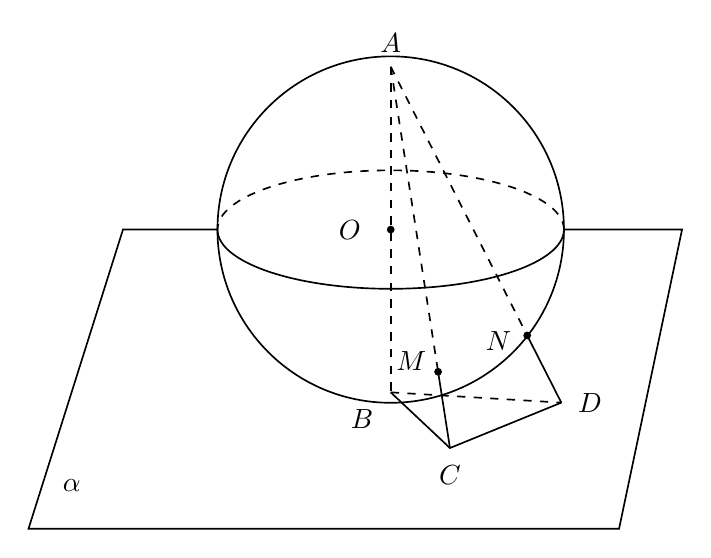
\begin{tikzpicture}[x=1cm,y=1cm,font=\normalsize,line width=.6pt]
\coordinate (A) at (0,2.967323766);
\coordinate (O) at (0,0.90);
\coordinate (B) at (0,-1.167323766);
\coordinate (C) at (0.7524443153,-1.874390136);
\coordinate (D) at (2.166577057,-1.29798435);
\coordinate (M) at (0.6019554523,-0.906047356);
\coordinate (N) at (1.733261645,-0.4449227268);
% sphere outline
\draw[solid] (O) circle (2.20);
% equator: front solid, back dashed
\draw[solid] (2.20,0.90) arc [x radius=2.20,y radius=0.7524443153,start angle=0,end angle=-180];
\draw[dashed] (2.20,0.90) arc [x radius=2.20,y radius=0.7524443153,start angle=0,end angle=180];
% plane alpha (back edge meets equator ends, extends outward)
\draw[solid] (-2.20,0.90) -- (-3.40,0.90) -- (-4.60,-2.90) -- (2.90,-2.90) -- (3.70,0.90) -- (2.20,0.90);
% triangle BCD on plane
\draw[solid] (B) -- (C) -- (D);
\draw[dashed] (B) -- (D);
% AC split at M, AD split at N
\draw[dashed] (A) -- (M);
\draw[solid] (M) -- (C);
\draw[dashed] (A) -- (N);
\draw[solid] (N) -- (D);
% diameter AB
\draw[dashed] (A) -- (B);
% dots
\fill (O) circle (1.4pt);
\fill (M) circle (1.4pt);
\fill (N) circle (1.4pt);
% labels kept clear of strokes
\node[inner sep=2pt,above=3pt] at (A) {$A$};
\node[inner sep=2pt,anchor=east] at (-0.30,0.90) {$O$};
\node[inner sep=2pt,below left=4pt] at (B) {$B$};
\node[inner sep=2pt,left=2pt,xshift=0.00bp,yshift=4.00bp] at (M) {$M$};
\node[inner sep=2pt,left=3pt,yshift=-2pt,xshift=-0.5bp,yshift=-0.0bp] at (N) {$N$};
\node[inner sep=2pt,below=4pt] at (C) {$C$};
\node[inner sep=2pt,anchor=west] at (2.30,-1.30) {$D$};
\node[inner sep=2pt] at (-4.05,-2.35) {$\alpha$};
\end{tikzpicture}
